\documentclass[openright]{memoir}

\usepackage{amsmath}
\usepackage{graphicx}
\usepackage{xcolor}
\usepackage{ragged2e}
\usepackage{tikz}
\usetikzlibrary{calc}
\usepackage{blindtext}
\usepackage{xparse}

% Page size settings
\setulmarginsandblock{70pt}{50pt}{*}
\setlrmarginsandblock{90pt}{90pt}{*}
\setheadfoot{\baselineskip}{\baselineskip}
\setheaderspaces{28pt}{*}{*}
\checkandfixthelayout

\maxtocdepth{subsection}

% Set up chapter ToC
\newcounter{tocmarker}
  \renewcommand\mempreaddchaptertotochook{\cftinserthook{toc}{end-\thetocmarker}}
  \renewcommand\mempreaddparttotochook   {\cftinserthook{toc}{end-\thetocmarker}}
  \renewcommand\mempreaddbooktotochook   {\cftinserthook{toc}{end-\thetocmarker}}
  \renewcommand\mempreaddapppagetotochook{\cftinserthook{toc}{end-\thetocmarker}}
  % start marker
  \renewcommand\mempostaddchaptertotochook{%
    \stepcounter{tocmarker}\cftinserthook{toc}{start-\thetocmarker}}
  \let\normalchangetocdepth\changetocdepth % for later


\makeatletter
\newcommand\chaptertoc{
  % make changes local, remember counters a global
  \begingroup
  % store current value, to be restored later
  \setcounter{@memmarkcntra}{\value{tocdepth}}
  % when ever \settocdepth is used, it adds the new value to the
  % ToC data. This cause problems when we want to disable all
  % entries. Luckily the data is added via a special macro, we we
  % redefine it, remember we stored the original value earlier.
  \let\changetocdepth\@gobble
  % disable all entries (using our copy from above)
  \normalchangetocdepth{-10}
  % enable toc data within our block, we go as far as subsubsection
  \cftinsertcode{start-\thetocmarker}{\normalchangetocdepth{1}}
  % when the block is done, disable the remaining
  \cftinsertcode{end-\thetocmarker}{\normalchangetocdepth{-10}}
  % remove the spacing above the toc title
  \let\tocheadstart\relax
  % remove the toc title itself
  \let\printtoctitle\@gobble
  % remove space below title
  \let\aftertoctitle\relax
  % reformat TOC entries:
  \setlength{\cftsectionindent}{0pt}
  \setlength{\cftsubsectionindent}{\cftsectionnumwidth}
  \setlength{\cftsubsubsectionindent}{\cftsubsectionindent}
  \addtolength{\cftsubsubsectionindent}{\cftsubsectionnumwidth}
  \renewcommand\cftsectionfont{\small}
  \renewcommand\cftsectionpagefont{\small}
  \renewcommand\cftsubsectionfont{\small}
  \renewcommand\cftsubsectionpagefont{\small}
  \renewcommand\cftsubsubsectionfont{\small}
  \renewcommand\cftsubsubsectionpagefont{\small}
  % include the actual ToC data
  \tableofcontents*
  \endgroup
  % restore tocdepth
  \setcounter{tocdepth}{\value{@memmarkcntra}}
  % to indent or not after the chapter toc
  \m@mindentafterchapter
  % space between chapter toc and text
  \par\bigskip
  % handles indentation after the macro
  \@afterheading}
\makeatother

\aliaspagestyle{frontps}{plain}

% Extend header to cover marginal notes.
\setlength{\headwidth}{\textwidth}
   \addtolength{\headwidth}{\marginparsep}
   \addtolength{\headwidth}{\marginparwidth}

% Page style memst
\makeatletter
\makepagestyle{memst}
\makerunningwidth{memst}{\headwidth}

\makeevenhead{memst}{%
  \sffamily\bfseries\thepage\quad\mdseries\leftmark}{}{}
\makeoddhead{memst}{}{}{\sffamily\mdseries\rightmark\quad\bfseries\thepage}

\makepsmarks{memst}{%
  \def\chaptermark##1{%
    \markboth{\MakeUppercase\@chapapp\ \thechapter\ |\ \ ##1}{}}
  \def\sectionmark##1{%
    \markright{\color{secnumcolor}SECTION \thesection\ |\ ##1}}}
\makeatother

% Chapter style memst
\makechapterstyle{memst}{%
  \definecolor{chapcolor}{RGB}{0,5,73}
  \renewcommand*{\chaptitlefont}{\color{chapcolor}\sffamily\Huge}
  \renewcommand*{\printchaptername}{}
  \renewcommand*{\printchapternum}{}
  \renewcommand*{\afterchaptertitle}{%
    \par\nobreak\vskip5pt\hrule\vskip\afterchapskip}
}

% Section style
\definecolor{secnumcolor}{RGB}{49,55,138}
\definecolor{sectitlecolor}{RGB}{119,116,78}
\newcommand{\ruledsec}[1]{%
  \color{sectitlecolor}\Large\mdseries\scshape\raggedright#1%
  \vskip-0.6\baselineskip\rule{\textwidth}{0.4pt}}
\setsecheadstyle{\ruledsec}
\setsecnumformat{\color{secnumcolor}\bfseries\csname the#1\endcsname\quad}


\ExplSyntaxOn 
\NewDocumentCommand \completechapterpage { m }
{
  \chaptertoc
  \RaggedRight #1
  \clearpage
}
\ExplSyntaxOff


\begin{document}

\frontmatter

\pagestyle{frontps}
\chapterstyle{default}

\newlength{\mylength}
\calccentering{\mylength}
\begin{adjustwidth*}{\mylength}{-\mylength}
\tableofcontents*\thispagestyle{frontps}
\newpage
\listoffigures\thispagestyle{frontps}
\end{adjustwidth*}

\mainmatter

\pagestyle{memst}
\chapterstyle{memst}

\chapter{Fundamentals} \completechapterpage{Perhaps the most useful idea for
    modeling the real world is the concept of \emph{function}. Let's look at an
        example. If a rock climber drops a stone from a high cliff, we know
        that the stone will fall. But this general description doesn't help us
        figure out when the stone will hit the ground. To find out, we need a
        \emph{rule} that relates the distance $d$ the stone falls to the time
        it has been falling. Galileo was the first to discover the rule: In $t$
        seconds the stone falls $16t^2$ feet. This “rule” is called a
        \emph{function}; we write this function as $d(t) = 16t^2$. Using this
        function model, we can \emph{predict} when the stone will hit the
        ground. In this chapter we study properties of functions and how
        function models can help us to get precise information about the thing
        or process being modeled.}

\section{What is a Function?}

A function is a rule.\sidepar{\itshape We have previously used letters to stand
    for numbers. Here we do something quite different: We use letters to
        represent rules.} To talk about a function, we need to give it a name.
        We will use letters such as $f$, $g$, $h$, $\ldots$ to represent
        functions.

\Blindtext[3]

\section{Graphs of Functions}

The graph of a
function\marginpar{\raisebox{-\height}{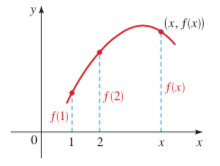
\includegraphics[width=\marginparwidth]{figure2}}}
$f$ gives a picture of the behavior or “life history” of the function. We can
read the value of $f(x)$ from the graph as being the height of the graph above
the point $x$.

\Blindtext[2]

\section{Getting Information from the Graph of a Function}

\blindmathpaper

\section{Average Rate of Change of a Function}

\subsection{Average Rate of Change}

We are all familiar with the concept of speed: If you drive a distance of 120
miles in 2 hours, then your average speed, or rate of travel, is $\frac{120
    mi}{2 h} = 􏱁 60 mi/h$. Now suppose you take a car trip and record the
    distance that you travel every few minutes. The distance $s$ you have
    traveled is a function of the time $t$: \[ s(t) = \text{total distance
        traveled at time } t \] We graph the function $s$ as shown in
        \fref{fig:1}. The graph shows that you have traveled a total of 50
        miles after 1 hour, 75 miles after 2 hours, 140 miles after 3 hours,
        and so on. To find your average speed between any two points on the
        trip, we divide the distance traveled by the time elapsed.

\begin{figure} \centering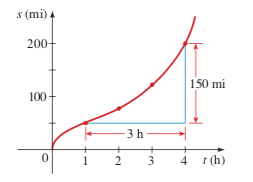
\includegraphics[scale=.6]{figure1} \caption{Average
    speed}\label{fig:1} \end{figure}

\Blindtext

\chapter{Polynomial and Rational Functions} \completechapterpage{Functions
    defined by polynomial expressions are called polynomial functions.  The
        graphs of polynomial functions can have many peaks and valleys; this
        makes them suitable models for many real-world situations.  For
        example, a factory owner notices that if she increases the number of
        workers, productivity increases, but if there are too many workers,
    productivity begins to decrease.  This situations is modeled by a
        polynomial function of degree 2 (a quadratic function).  As another
        example, when a volleyball is hit, it goes up and then down, following
        a path that is also modeled by a quadratic function.  The graphs of
        polynomial functions are smooth curves that are used in designing many
        things. For example, sailboat designer put together portions of the
        graphis of different cubic functions (called cubic splines) to make the
        curves of the hull of a sailboat.}


\section{Quadratic Functions and Models}

\blindtext

\section{Polynomial Functions and Their Graphs}

\blindmathpaper

\section{Dividing Polynomials}

\Blindtext

\section{Real Zeros of Polynomials}

\blindmathpaper

\section{Complex Numbers}

\blindtext \Blindlist{enumerate}

\chapter{Exponential and Logarithmic Functions}
\completechapterpage{\blindtext[1]}

\section{Exponential Functions}

\blindmathpaper

\section{The Natural Exponential Function}

\Blindlist{description}

\section{Logarithmic Functions}

\Blindlist{itemize}

\section{Laws of Logarithms}

\Blindtext

\end{document}
